\chapter{Discussion : interprétation conjointe des transitions de réversibilité et d'écoulement}

\label{chapter:discussion}

\subparagraph{}Dans ce chapitre, nous proposons de rassembler les résultats obtenus dans les chapitres précédents afin de mener une étude comparée de la transition de réversibilité et de la transition vers l'écoulement. Nous nous appuierons tout d'abord sur les modèles numériques étudiés pour formuler plus précisément l'analogie entre les deux systèmes, du point de vue microscopique comme du point de vue de la modélisation en champ moyen. Nous montrerons alors l'importance donnée aux mécanismes de bruit interne présents dans ces deux phénomènes.

\subparagraph{}Nous comparerons ensuite les évolution mesurées dans les modèles numériques de la criticalité de ces transitions avec la portée de l'interaction. Pour ce faire, nous nous appuierons essentiellement sur l'évolution de la convexité associée, soit l'exposant critique $\beta$. Si celle-ci suit des évolutions globalement similaires dans les deux cas, nous proposerons un scénario et ses limites pour expliquer les points de divergence qui subsisitent. Celui-ci se basera sur les ingrédients de la dynamique présents dans les modèles microscopiques.

\section{Des similarités globales}

\subsection{Analogie entre les deux systèmes}

\subparagraph{}Après avoir présenté une étude exhaustive des deux transitions via les modèles numériques évoqués aux chapitres précédents, nous proposons de revenir sur les conclusions du \autoref{chapter:introduction} pour reformuler plus précisément l'analogie entre les deux systèmes. Dans le \autoref{tab:analogie}, nous développons les parallèles réalisables entre ces deux transitions représentées par les modèles du $\alpha$-ROM et du $\alpha$-Picard.

\subsubsection{Activité et quantité conservée}

\subparagraph{}\`A l'instar des modèles appartenant à la classe CDP, les modèles $\alpha$-ROM et $\alpha$-Picard font tout deux intervenir la dynamique d'une activité et d'une quantité conservée. Concernant la quantité conservée, elle correspond à la contrainte locale $\sigma(\mathbf{r},t)$ dans le $\alpha$-Picard, qui est l'équivalent de la densité de particules $\rho(\mathbf{r}, t)$ dans le $\alpha$-ROM. Cette première analogie rappelle directement le parallèle entre la transition de dépiégeage et les modèles de particules appartenant à la classe CDP\footnote{Dans le \autoref{chapter:introduction}, nous avons présenté une équivalence entre la force élastique de rappel locale dans la transition de dépiégeage et la densité de particules dans le modèle Manna}. Du côté de l'activité, une analogie directe est établie entre l'activité gros grains $A(\mathbf{r}, t)$ dans le $\alpha$-ROM et la variable locale $\dot{\epsilon}_\text{pl}(\mathbf{r}, t)$ dans le modèle $\alpha$-Picard.

\subparagraph{}Dans les deux cas, et comme dans tous les modèles représentés par l'universalité CDP, la valeur locale du champ conservé correspond en quelque sorte à une susceptibilité à l'activation. Une densité élevée dans le $\alpha$-ROM correspond à des particules proches, i.e. susceptibles de se recouvrir suite à un petit déplacement et donc de créer de l'activité. Dans le modèle $\alpha$-Picard, une contrainte locale élevée représente une faible distance au seuil microscopique $\sigma_Y$ et donc une éventualité forte de devenir plastique en la présence de fluctuations externes.

\subparagraph{}D'un point de vue macroscopique, les paramètres de contrôle homologues l'un de l'autre sont la contrainte globale $\Sigma$ et la densité globale $\phi$, tandis que l'équivalence des paramètres d'ordre se retrouve via la proportion moyenne de particules actives $\langle A \rangle $ et le taux de cisaillement moyen $\langle \dot{\gamma}\rangle$.

\subsubsection{Avalanches et hyperuniformité}

\subparagraph{}Comme les autres modèles appartenant à la classe CDP, le $\alpha$-ROM et le modèle $\alpha$-Picard présentent des dynamiques d'avalanche proche du point critique, que nous avons mises en évidence dans des conditions de contrainte/densité imposée. En accord avec les équivalences précédentes, là où la taille d'une avalanche dans le modèle $\alpha$-Picard est représentée par le déplacement global du matériau, celle dans le $\alpha$-ROM correspond à la quantité d'évènements actifs qui la constituent. De même, on retrouve dans ces deux systèmes, dans une certains limite, la propriété d'hyperuniformité. Si celle-ci se traduit dans le modèle de particules via les fluctuations anormales de densité, dans le modèle d'écoulement elle correspond aux fluctuations anormales de contrainte.

\subsubsection{Effets multiples des évènements d'activité}

\subparagraph{}L'analogie entre les deux modèles peut être complété plus spécifiquement en s'intéressant à  l'effet d'un évènement actif dans le système. Celui-ci peut en fait être découpé en trois contributions : un effet de relaxation (0), un effet de transport (1) et un effet non-local spécifique (2) qui fait la particularité des transitions étudiées. Par transport, nous entendons ici, comme dans le \autoref{chapter:introduction}, un déplacement de la quantité conservée à l'échelle microscopique issu d'une zone d'activité. Cette notion de transport représente donc le mécanisme classique de propagation de l'activité dans les modèles appartenant à la classe CDP. Nous verrons par la suite que ce découpage est utile pour comprendre les différents mécanismes à l’œuvre dans chacune de ces transitions.

\subparagraph{}Pour clarifier cette division, prenons tout d'abord le cas du $\alpha$-ROM. Dans ce modèle, le processus de relaxation (0) se traduit par le saut de la particule active. En effet, en réalisant ce saut la particule active défait le recouvrement qui avait mené à son activation. C'est donc bien un processus d'auto-inhibition local de l'activité. D'autre part, le processus de transport (1) correspond au déplacement de la particule active qui est susceptible d'en recouvrir une autre. Il correspond alors exactement au même mécanisme de transport que celui présent dans le ROM. Il est donc fait à courte portée. Enfin, le processus non-local spécifique (2), qui le différencie des autres modèles associés au ROM, est l'interaction entre particules actives et passives à longue portée, représentée par des petits déplacements des particules passives sans transport des particules actives. 

\subparagraph{}Dans le cas du modèle $\alpha$-Picard, ce découpage est un peu moins évident mais peut être compris par une ré-écriture formelle du propagateur selon :

\begin{equation}
	G(\mathbf{r}-\mathbf{r}^\prime) = G(0) + G_1(\mathbf{r}-\mathbf{r}^\prime) + G_2(\mathbf{r}-\mathbf{r}^\prime), \quad \int \mathrm{d}\mathbf{r}~ G_1(\mathbf{r}) = -G(0)
\end{equation}

\noindent $G_1$ définissant la partie isotrope du propagateur. Dans le cas des modèles $\alpha$-Picard, dans la limite continue, celui-ci prend la forme :

\begin{equation}
	G_1(r) = B_\alpha\frac{C_\alpha}{r^\alpha}
\end{equation}

\noindent avec $C_\alpha$ et $B_\alpha$ des constantes définies par l'\autoref{eq:RealAlphaPicard} au \autoref{chapter:yielding}. Dans les cas spécifiques $\alpha = 2$ et $\alpha = 4$, le terme $C_\alpha$ s'annule. Toutefois, dans un système fini, la conservation de la contrainte globale implique nécessairement l'existence d'un tel terme. En pratique, celui-ci prend plutôt une forme uniforme qui se comporte comme $\sim 1/L^2$ dans le cas spécifique $\alpha = 2$. Pour $\alpha = 4$, la partie isotrope du propagateur discret implémenté est moins évidente. (\rem{mieux vaut ne rien dire sur ces cas spécifiques si on n'a pas grand chose à en dire ?}).


\subparagraph{}Dans le cadre du modèle $\alpha$-Picard, le processus de relaxation (0) correspond à la partie $G(0)<0$ du propagateur qui traduit la relaxation d'un site plastique, l'amenant vers $\sigma < \sigma_Y$ et donc vers le retour à un état élastique. Le processus de transport (1), quant à lui, correspond à la redistribution de cette contrainte relaxée via la partie isotrope du propagateur $G_1$. Dans le cas de la transition de dépiégeage, le propagateur élastique n'est formé que des deux premiers termes. La particularité du propagateur non-monotone d'Eshelby dans le cas de la transition vers l'écoulement fait intervenir un troisième terme $G_2$, à longue portée et de signe alterné. C'est cette partie qui représente l'effet non-local spécifique (2) de la transition, absent des modèles représentant les classes CDP et LR-CDP. En effet, celui-ci ne peut pas être traduit comme le déplacement de la contrainte relaxée vers d'autres sites.

\subparagraph{}L'ingrédient constitutif qui rapproche les deux transitions de réversibilité et d'écoulement et les sépare des classes CDP et LR-CDP est précisément cette partie non-locale spécifique (2) de l'effet de l'activité. Dans la suite, nous rappelons brièvement en quoi celle-ci représente un nouveau mécanisme de création de l'activité, par opposition au mécanisme usuel de création de l'activité par transport dans les classes CDP et LR-CDP.

\begingroup

\setlength{\tabcolsep}{10pt}
\renewcommand{\arraystretch}{1.5}

\begin{table}[h]
\centering
\begin{tabular}{P{0.25\linewidth}P{0.35\linewidth}P{0.35\linewidth}}
\hline \hline  & $\alpha$-ROM & $\alpha$-Picard \\
\hline
Param. de contrôle  & densité $\phi$ & contrainte $\Sigma$ \\
Param. d'ordre & fraction de particules actives $A$ & taux de cisaillement $\dot{\gamma}$ \\
Mise en activité & contact : $|\mathbf{r}-\mathbf{r}^\prime| < D_P$ & dépassement du seuil : $\sigma > \sigma_Y$\\
Effet local de l'act. & saut & relaxation de $\sigma$ \\
Effet non-local de l'act. & déplacement local des part. passives & modification des contraintes locales à longue portée \\
Distribution de distance micro.  & fonction de corrélation de paire : $g_p(|\mathbf{r}-\mathbf{r}^\prime|-D_p)$ & distribution de distance au seuil : $P(\sigma_Y - \sigma)$\\
\hline 
Présence de transport à longue portée & Non (sauts à courte portée) & Oui (via la partie $G_1$ du propagateur) \\
Géométrie du propagateur & isotrope & présence de modes 0 \\
\hline \hline
\end{tabular}
\caption{Tableau d'analogie entre la transition de réversibilité et la transition vers l'écoulement étudiées via les modèles $\alpha$-ROM et $\alpha$-Picard.}
\label{tab:analogie}
\end{table}

\endgroup

\subsection{Bruit interne, bruit mécanique}

\subsubsection{Diffusion vers une barrière}

\subparagraph{}Dans le modèle $\alpha$-ROM, comme nous l'avons discuté au \autoref{chapter:Susp}, l'effet non-local spécifique des interactions à longue portée provoque une diffusion des particules passives via l'effet successif de nombreux évènements actifs. Cette diffusion représente alors un mécanisme de propagation de l'activité très différent de celui des modèles associés à la classe CDP. Sous l’influence du bruit interne, les particules passives se déplacent aléatoirement et finissent par se rencontrer. Ainsi, à partir de deux particules passives, deux particules actives sont créées, tandis que les particules actives à l'origine de ce bruit interne poursuivent leur dynamique purement locale. Formellement, ce mécanisme de création de l'activité peut être associé à une marche aléatoire en présence d'une barrière. Dans le $\alpha$-ROM, pour une particule passive, cette barrière est représentée par toute autre particule. L'activation de la particule suite au franchissement de cette barrière correspond alors au mécanisme de création d'activité associé à ce bruit interne.

\subparagraph{}Le même constat peut être fait du point de vue des modèles élastoplastiques en considérant l'effet de la partie $G_2$ du propagateur. Si l'on se concentre sur un site élastique lors d'un pas de temps unique, en fonction de sa position relative à la plasticité, sa contrainte locale se voit augmenter ou diminuer de manière plus ou moins importante (du fait que $G_2$ soit de signe alterné). Au cours de l'écoulement, via les fluctuations de plasticité dans le système, la contrainte locale de ce site va donc fluctuer de manière pseudo-aléatoire. Nous utilisons ici le terme pseudo-aléatoire puisque, en pratique, la modification de la contrainte suite à un rérrangement plastique est déterministe. Seulement, la stochasticité de la contrainte locale relaxée et les corrélations finies du champ de plasticité permettent de comprendre ces interactions comme une sorte de bruit effectif au niveau local. Dans ce cadre, nous pouvons donc voir l'effet non-local spécifique des modèles $\alpha$-Picard comme induisant une diffusion des contraintes locales. Là encore, cette diffusion définit un nouveau mécanisme de création d'activité qui peut être compris comme une marche aléatoire en présence d'une barrière. La contrainte locale $\sigma$ diffuse sous l'action de la plasticité jusqu'à arriver au seuil $\sigma_Y$ qui représente la barrière, créant ainsi de l'activité dans le système. 

\subparagraph{}Ces mécanismes de diffusion vers un bord absorbant sont complexes à appréhender en dimension finie car ils ne peuvent pas être réellement réduit à un problème de marche aléatoire simple. Dans le cas du $\alpha$-ROM, cela vient du fait que les particules actives qui créent le bruit interne opèrent une dynamique corrélée non-triviale et que la notion de barrière ne renvoie pas à une frontière fixe mais à un ensemble de particules diffusant elles aussi dans un espace de dimension finie. Dans le cas du modèle $\alpha$-Picard, l'effet du propagateur $G_2$ n'est que pseudo-aléatoire puisqu'il présente une forte anisotropie quadrupolaire en plus d'une spatialisation. Pour ces raisons, il est plus simple d'aborder ce mécanisme dans un premier temps via un point de vue champ moyen qui permet de s'affranchir de toutes ces sources de complexité. 

\subsubsection{Modélisation champ moyen}

\subparagraph{}Il est possible d’interpréter les deux transitions via des modèles de champ moyen comprenant ce mécanisme non-local spécifique de la manière la plus simple qu'il soit. Ceux-ci se démarquent des approches champ moyen issues des équations de champ comme dans le cas de CDP par deux aspects : l'objet central de la théorie est le champ conservé et non le champ d'activité, et le point de vue adopté est un point de vue mésoscopique/microscopique, via la dynamique effective d'un agent unique.

\subparagraph{}Dans le cadre de la transition vers l'écoulement, ce modèle champ moyen est le modèle de Hébraud-Lequeux \cite{hebraud_mode-coupling_1998}, décrit par l'équation :

\begin{equation}
\begin{aligned}
	\partial_t P(\sigma, t) &= -\dot{\gamma}(t)\partial_\sigma P(\sigma, t) + a\Gamma(t)\partial_\sigma^2P(\sigma, t) - \frac{\Theta (|\sigma|>\sigma_Y)}{\tau}P(\sigma, t) + \Gamma(t)\delta(\sigma)\\
	\Gamma(t) &= \frac{1}{\tau}\int_{|\sigma|>\sigma_Y}\mathrm{d}\sigma ~ P(\sigma, t)
\end{aligned}
\end{equation}

\noindent avec $\dot{\gamma}(t) = \dot{\gamma}$ dans des conditions de taux de cisaillement imposé ou alors :

\begin{equation}
	\dot{\gamma} (t) = \frac{1}{\tau}\int_{|\sigma|>\sigma_Y}\mathrm{d}\sigma ~ \sigma P(\sigma, t)
\end{equation}

\noindent dans le cas où c'est la contrainte globale $\Sigma = \int \mathrm{d}\sigma ~ \sigma P(\sigma,t)$ qui est imposée.

\subparagraph{}Dans le cas de la transition de réversibilité, le modèle équivalent est décrit par les équations présentées au \autoref{chapter:Susp} :

\begin{equation}
\begin{aligned}
    \partial_t P(\mathbf{r}, t) &= a\Gamma (t)\nabla^2 P(\mathbf{r}, t) - \frac{1}{\tau}\Theta(|\mathbf{r}|>R)P(\mathbf{r}, t) + \delta(\mathbf{r})\Gamma (t)\\
     \Gamma (t) &= \frac{1}{\tau}\int_{|\mathbf{r}|>R}\mathrm{d}\mathbf{r}~P(\mathbf{r}, t)
    \label{eq:muHLDiffdisc}
\end{aligned}
\end{equation} 

\subparagraph{}Là où le lien avec la modélisation élastoplastique du modèle $\alpha$-Picard est complètement transparent, celui avec le $\alpha$-ROM demande un certain degré d'abstraction et d'hypothèse via la mise en place d'une cage effective de dimension $R$, comme nous l'avons présenté au \autoref{chapter:Susp}. En fait, si le lien est plus direct dans le cadre de la transition vers l'écoulement c'est parce que les modèle élastoplastiques ont déjà intégré ce degré d'abstraction dans leur construction, à la différence de modèle plus maximaux comme les simulations de dynamique moléculaire. Ceci fait, les équations régissant cette image champ moyen sont très similaires et permettent de comprendre les interactions à longue portée de la même façon via les termes en laplacien : chaque élément est soumis à un bruit dont l'intensité est proportionnelle à l'activité dans le système. Par ailleurs tout élément ayant dépassé la barrière ($R$ ou $\sigma_Y$) est considéré comme actif.

\subparagraph{}La différence fondamentale entre ces deux modèles est la présence d'un terme de forçage en $\sim \dot{\gamma}$ dans le modèle de Hébraud-Lequeux, absent dans l'équivalent pour la transition de réversibilité, et la dimension dans laquelle prend place la diffusion. Toutefois, en considérant les paramètres de contrôle respectifs ($\Sigma = \int \mathrm{d}\sigma ~ \sigma P(\sigma,t)$ dans le cas de la transition d'écoulement et $R$ dans le cas de la transition de réversibilité), ces deux modèles prédisent un même comportement critique représenté par un exposant $\beta = 2$ :

\begin{equation}
	\Gamma \sim (\Sigma - \Sigma_c)^2,\quad \Gamma \sim (R_c-R)^2
\end{equation}

\noindent Ces modèles renforcent alors l'analogie entre les deux transitions et placent ainsi le mécanisme de création de l'activité par diffusion (des particules passives dans la transition de réversibilité et des contraintes locales dans la transition vers l'écoulement) comme l'explication de la convexité observée dans les modèles de dimension finie.

\paragraph{Extension à l'influence de la portée des interactions}

\subparagraph{}Comme on l'a vu dans le cas des suspensions au \autoref{chapter:Susp}, il est possible d’interpréter l'influence de la portée des interactions dans ce cadre champ moyen en considérant que celle-ci dicte les propriétés du bruit interne, plus précisément sa distribution. Cela se traduit dans les équations des modèles par un remplacement du laplacien classique $\nabla^2$ en un laplacien fractionnaire $-|\nabla|^\mu$. Dans le modèle d'écoulement, cette généralisation a été étudiée précédemment par Lin et al. \cite{lin_mean-field_2016, lin_microscopic_2018}, montrant une évolution de la convexité avec $\mu$ décrite par :

\begin{equation}
	\beta = \left\{
	\begin{aligned}
	&2, \quad \mu > 2\\
	&\mu, \quad 1<\mu<2\\
	&1, \quad \mu < 1
	\end{aligned}
	\right.
\end{equation}

\noindent et la présence de corrections logarithmiques dans le cas limite $\mu = 1$\footnote{Dans ce cas là nous avons $\delta\Sigma \sim \dot{\gamma}\log(\dot{\gamma})$}. Dans l'approximation où le système est exempt de toutes corrélations liées à la dimension du système, l'équivalence discutée au \autoref{chapter:Susp} entre $\mu$ et $D/\alpha$ suggère que les interactions à longue portée influent sur le comportement critique entre $\alpha = D$ et $\alpha = D/2$ avec $\beta$ passant de $\beta = 1$ à $\beta = 2$. Nous avons alors montré dans ce manuscrit que ces résultats se transposaient aussi au modèle champ moyen de particules. Cela suggère que l'influence de la portée des interactions est en principe le même dans les deux cas, du moins en ce qui concerne le mécanisme de création de l'activité par diffusion dans une approche champ moyen.

\subparagraph{}Ce cadre théorique qui permet d'expliquer l'évolution globale de la convexité sert alors d'appui pour interpréter les résultats obtenus dans les simulations de dimension finie et comparer plus quantitativement les deux transitions. C'est ce que nous ferons plus en détail à la \autoref{sec:Diff}.

\subsection{Répartition de la masse et distance à l'activation : des indices microscopiques}

\subparagraph{}En plus de la convexité des transitions, une preuve de l'importance du mécanisme de diffusion pour la création d'activité dans les modèles $\alpha$-ROM et $\alpha$-Picard vient des distributions de distances à l'activation.

\subparagraph{}Dans le cadre champ moyen commun aux deux transitions, nous pouvons définir une distance à l'activation associée à la dynamique à agent unique étudiée. Dans le cas du modèle d'écoulement, cette distance à l'activation est la distance à la contrainte seuil $x = \sigma_Y - \sigma$. Dans le cas du modèle pour la transition de réversibilité, c'est la distance au bord de la cage effective $x = R-|\mathbf{r}|$. Proche de la transition, les modèles champs moyens prévoient une distribution algébrique de ces distances dictée par un exposant critique $\theta$ selon :

\begin{equation}
	P(x) \sim x^\theta, \quad \theta = \left\{
	\begin{aligned}
	&\frac{\mu}{2}, \quad 1 < \mu \leq 2\\
	&1, \quad \mu \geq 2
	\end{aligned}
	\right.
\end{equation}

\noindent le cas $\mu \leq 1$ dépendant de la présence ou non d'un forçage dans le modèle \cite{lin_mean-field_2016} (et donc différent dans le cas du modèle d'écoulement et du modèle pour la transition de réversibilité). Ce résultat place alors la mesure $\theta > 0.5$ en témoin de l'importance du mécanisme de diffusion dans la transition.

\subparagraph{}Par construction, il est possible de définir un équivalent de ces propriétés dans les modèles microscopiques. Dans le modèle $\alpha$-Picard, l'équivalence est directe avec la distribution $P(x)$, $x$ étant la distance au seuil définie sur chacun des $N$ sites. Dans le $\alpha$-ROM, nous avons associé au \autoref{chapter:Susp} cette distribution à la fonction $g(x)$ obtenue de la fonction corrélation de paire entre particules passives $g_p$ selon $g(x) = g_p(x = r - D_p)$.

\subparagraph{}Dans le cas du $\alpha$-ROM, nous avons montré que cette distribution était effectivement caractérisée par un exposant $\theta$ non-trivial évoluant avec la portée. Dans le cas du modèle élastoplastique, la quantité $P(x)$ a été étudiée à de nombreuses reprises, notamment car l'exposant $\theta$ est relié aux propriétés des avalanches quasistatiques \cite{lin_scaling_2014, ferrero_criticality_2019, liu_driving_2016, lin_mean-field_2016}. Dans ces études, on retrouve aussi dans le cas d'un propagateur de type Eshelby un exposant $\theta$ non-trivial entre $\theta = 0.5$ et $\theta = 1$. Notamment, dans le modèle de Picard que nous avons étudié, nous mesurons $\theta \approx 0.62$ (voir \autoref{sec:article2}). Cette propriété est un marqueur de la dynamique microscopique diffusive, absente dans les modèles de type CDP et depinning pour lesquels on a a priori $\theta = 0$ \cite{lin_scaling_2014} et conforte donc l'interprétation de ces transitions via le cadre de champ moyen commun proposé.

\subsection{Des évolutions qualitativement similaires dans les modèles numériques}

\subparagraph{}Dans une certaine mesure, l'évolution mesurée des criticalités du $\alpha$-ROM et du modèle $\alpha$-Picard avec la portée d'interaction $\alpha$ sont très similaires. Dans les deux cas, on passe continûment d'un comportement de courte portée similaire (ou équivalent) à la classe CDP à un comportement de très longue portée, similaire à celui proposé par les modèles de champ moyen de type Hébraud-Lequeux. Dans la limite de très longue portée, nous observons un comportement atypique dans les lois d'échelle régissant le régime stationnaire. L'évolution du paramètre d'ordre en fonction de la distance au point critique est convexe, caractérisée par un exposant $\beta$ proche de $2$, et les fluctuations de l'activité s'annulent à l'approche du point critique, caractérisées par un exposant $\gamma^\prime$ négatif.

\subparagraph{}Cette atypicité se traduit aussi dans les propriétés dynamiques des transitions, plus particulièrement via la dynamique d'avalanche à contrainte/densité imposée dans la limite de longue portée. Dans ce cas, les évènements perdent leur compacité spatiale, avec une extension spatiale caractérisée par un exposant $\chi$\footnote{Nous rappelons ici que l'exposant $\chi$ définit le comportement d'échelle entre la surface $A$ occupée par une avalanche et son extension spatiale $l$ selon $A\sim l^\chi$} inférieur à la dimension de l'espace $\chi < D$. De plus, nous observons dans les deux modèles que dans cette limite, les exposants $\chi$ et la dimension fractale des avalanches $d_f$ sont liés simplement par $d_f\approx \chi$. Le fait que la taille d'un évènement se comporte directement comme le nombre d'éléments impliqués suggère une sorte de simplification de la dynamique. L'évolution des propriétés critiques dynamiques repose alors essentiellement sur l'évolution de $\chi$ qui présente une perte de compacité supposée continue.

\subparagraph{}En fait, plus généralement, l'évolution de la plupart des exposants critiques prend la même forme que celle dans le cadre de la théorie LR-CDP : en augmentant la portée des interactions l'évolution du paramètre d'ordre devient moins concave, les fluctuations divergent de moins en moins fortement, les avalanches sont de moins en moins compactes, etc. Simplement, dans le cadre de ces deux transitions, la limite de longue portée est modifiée. Le mécanisme de création d'activité par diffusion, par opposition au mécanisme de création d'activité par transport, permet d'aller au-delà du comportement champ moyen de la classe CDP.

\subparagraph{}Une observation remarquable est que dans les deux cas, ce passage aux propriétés exotiques (convexité de la transition, annulation des fluctuations, perte de compacité des évènements, ...) se fait de manière simultanée pour tous les exposants. En d'autres termes, la limite de la région atypique est un point correspondant sous presque tous les aspects au comportement champ moyen de la classe CDP. Dans le cas du modèle $\alpha$-Picard, ce point est retrouvé autour de $\alpha \approx 3$. Pour le modèle $\alpha$-ROM, c'est autour de $\alpha \approx 1.5$. Il est possible que des relations d'échelle sous-jacentes permettent de rationaliser en partie cette simultanéité des différents passages $\beta > 1$, $\gamma^\prime < 0$, $\chi < D$. En revanche, il n'est toutefois pas clair qu'il existe une relation de cause à effet entre ces observations ou si elles représentent simplement une façon cohérente de caractériser cette dynamique. Quoiqu'il en soit, cette étude semble souligner le lien étroit entre convexité, évanescence des fluctuations et compacité de la dynamique. Dès lors, l'observation d'un élément de ce triptyque dans des systèmes différents pourrait suggérer la présence des deux autres propriétés, ou plus généralement la présence d'un mécanisme de création de l'activité par diffusion via la présence d'un bruit interne.

\newpage

\section{Des différences en dimension finie}

\subparagraph{}Si les modèles $\alpha$-Picard et $\alpha$-ROM sont similaires sous bien des aspects, leur étude détaillée aux \autoref{chapter:Susp} et \autoref{chapter:yielding} révèle des différences entre ces deux phénomènes. Dans cette sous-section, nous reprenons les approches théoriques présentées dans cette thèse pour proposer un scénario permettant d'expliquer les différences apparentes entre la criticalité du $\alpha$-ROM et celle du modèle $\alpha$-Picard. Pour ce faire, nous nous concentrerons sur une propriété centrale de ces transitions : leur convexité caractérisée par l'exposant critique $\beta$, dont nous reportons l'évolution sur la \autoref{fig:Recap}. Nous séparons ces différences, entre les deux modèles et entre les modèles et les approches théoriques, en deux catégories : celles de la zone concave $\beta < 1$ et celles de la zone convexe $\beta > 1$. Nous montrons alors que malgré ces divergences, l'interprétation de ces phénomènes dans un même cadre en dimension fini permet de mieux les appréhender. Enfin, nous discuterons des limites de cette interprétation.

\label{sec:Diff}

\subsection{Cadres d'interprétation théoriques}

\begin{figure}[h]
	\centering
	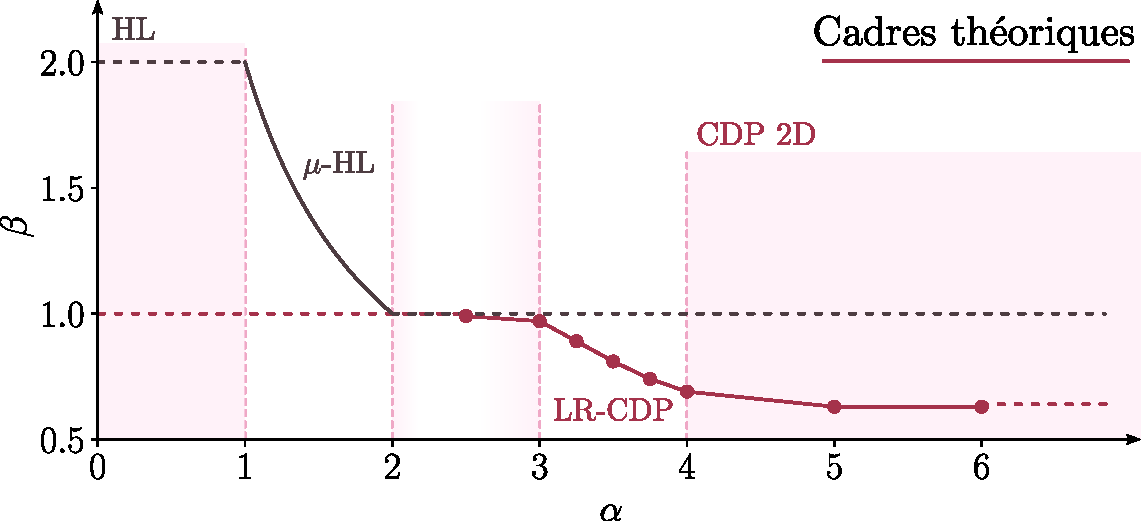
\includegraphics[width=\textwidth]{Chapitre5/Figures/RecapTheory.pdf}
	\caption{Evolution de l'exposant $\beta$ dans les cadres d'interprétation théorique LR-CDP et $\mu$-Hébraud-Lequeux avec $\mu = D/\alpha$. Les points correspondent aux mesures numériques sur le modèle LR-ROM (\autoref{chapter:TransportLP})}
	\label{fig:RecapTheory}
\end{figure}

\subparagraph{}Pour tenter de comprendre l'influence de la portée d'interaction sur le comportement critique dans les modèles $\alpha$-Picard et $\alpha$-ROM, nous disposons de deux approches théoriques. La première est celle présentée au \autoref{chapter:TransportLP}, baptisée LR-CDP, représentant l'influence du mécanisme de création de l'activité par transport à longue portée. En 2D, celle-ci prévoit une évolution continue des exposants entre $\alpha = 4$ et $\alpha = 3$, avec l'exposant $\beta$ allant de $\beta \approx 0.64$ à $\beta = 1$. La seconde est celle des modèles $\mu$-Hébraud-Lequeux qui, sous l'hypothèse $\mu = D/\alpha$, prédisent une évolution continue de la criticalité entre $\alpha=2$ et $\alpha = 1$ en 2D avec $\beta$ allant de $\beta = 1$ à $\beta = 2$. Nous représentons à la \autoref{fig:RecapTheory} la juxtaposition de ces deux approches qui opèrent sur des domaines de portée disjoints. Nous proposons alors de comparer les évolutions mesurées dans le $\alpha$-ROM et dans le $\alpha$-Picard sur cette base.

\begin{figure}[H]
	\centering
	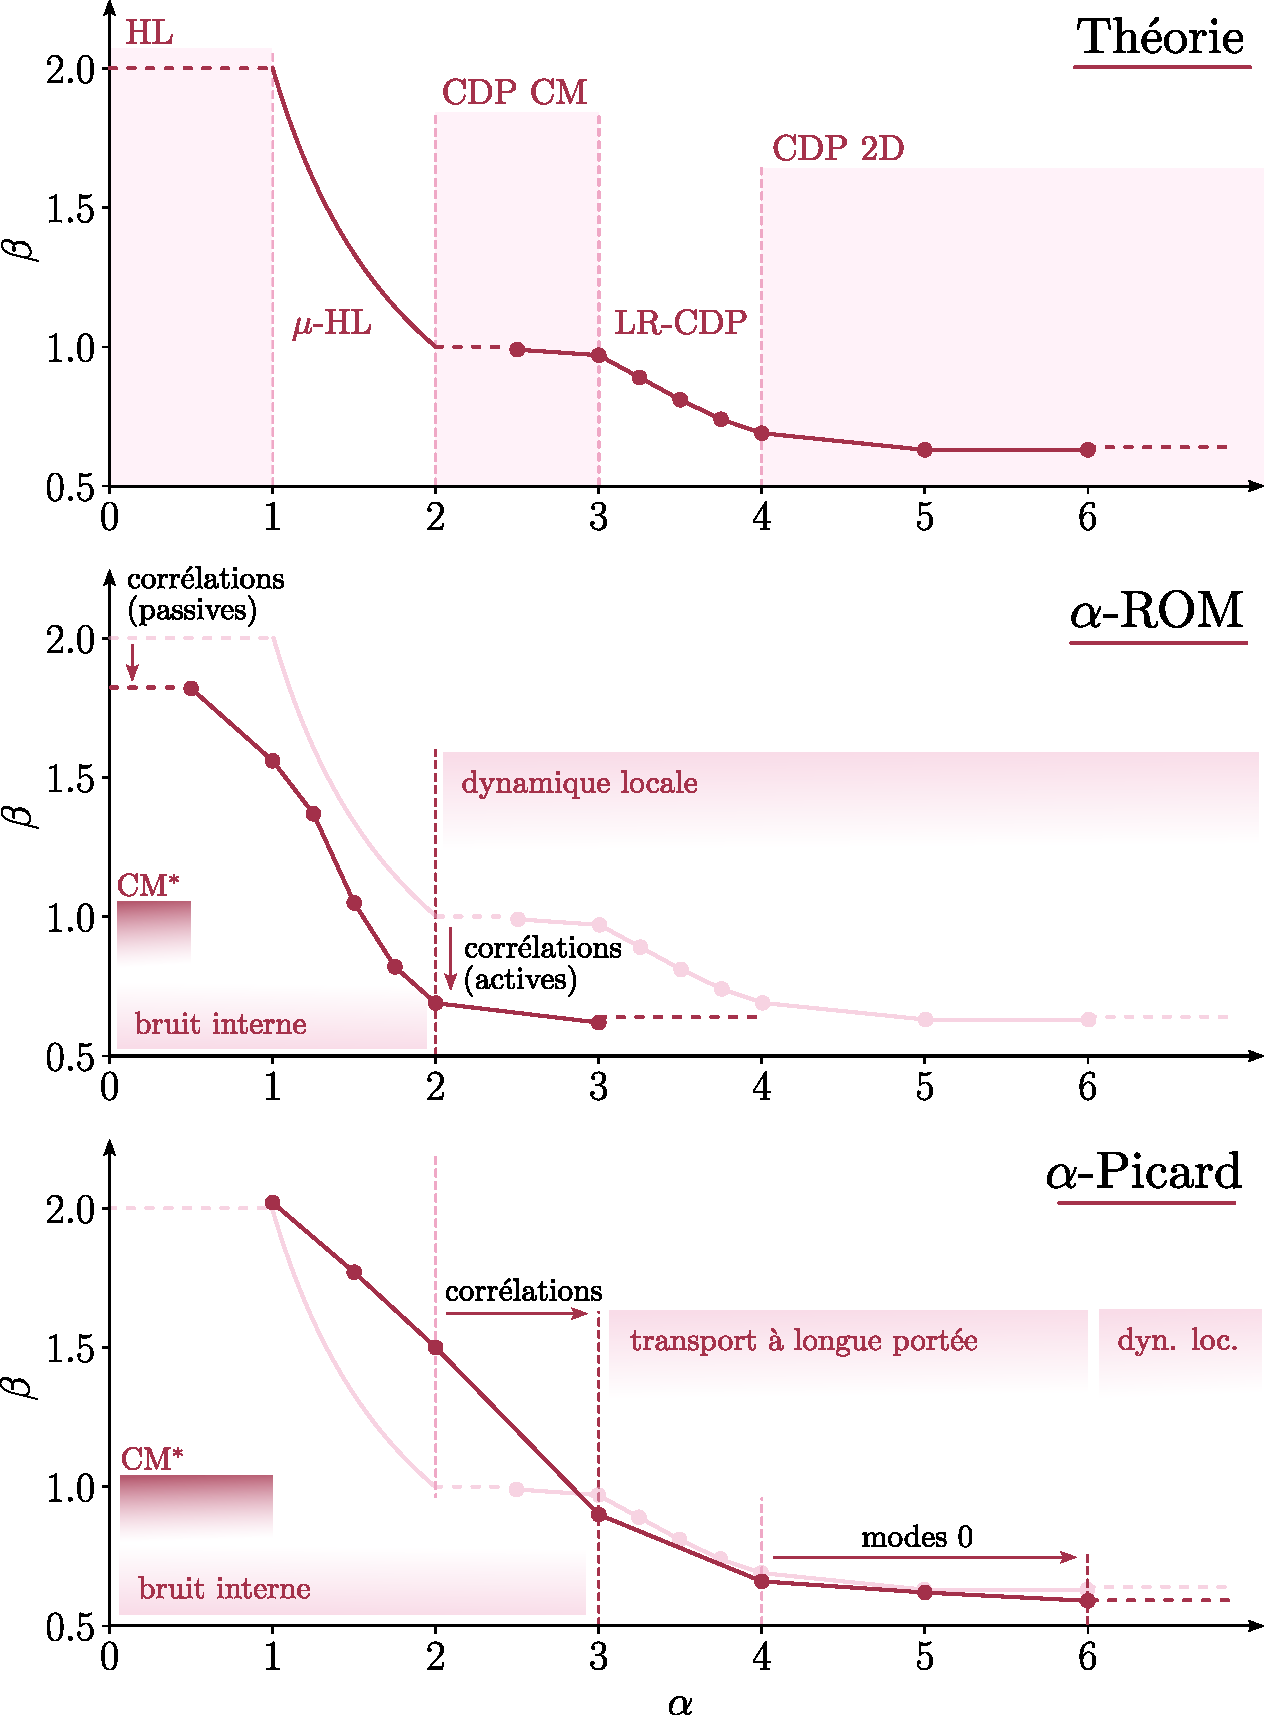
\includegraphics[width=\textwidth]{Chapitre5/Figures/FigRecap.pdf}
	\caption{Figure récapitulative de l'étude comparée des transitions de réversibilité et d'écoulement, représentée via le prisme de l'évolution de l'exposant $\beta$ avec la portée $\alpha$ en 2D. (b) Modèle $\alpha$-ROM (résultats du \autoref{chapter:Susp}). (c) Modèle $\alpha$-Picard (résultats du \autoref{chapter:yielding}). Les courbes roses en arrière-plan représente les évolutions présentées à la \autoref{fig:RecapTheory}.}
	\label{fig:Recap}
\end{figure}

\subsection{Zone concave : des évolutions décalées}

\subparagraph{}En comparant la \autoref{fig:Recap}-(a) et la \autoref{fig:Recap}-(b), une première différence est frappante : la gamme de portées pour laquelle la transition est concave n'est pas la même dans les deux cas. Dans le cas du modèle $\alpha$-Picard, celle-ci est définie par $\alpha \gtrsim 3$, avec une évolution très proche de celle du cadre LR-CDP, alors que dans le $\alpha$-ROM elle correspond à $\alpha \gtrsim 1.5$, montrant une évolution plus abrupte.

\subparagraph{}Dans le scénario que nous proposons, la différence de principe fondamentale entre les deux modèles qui explique le décalage de ce début d'évolution est à chercher du côté du mécanisme de création de l'activité par transport. Dans le cadre LR-CDP, l'évolution continue de la criticalité résulte d'une redstribution de masse (ou de contrainte) qui se fait à une portée de plus en plus étendue. Dans le modèle $\alpha$-Picard, cette propriété se retrouve dans la partie $G_1$ du propagateur qui correspond au transport de la contrainte localement relaxée, évoluant comme $\sim 1/r^\alpha$. Ceci explique l'accord qualitatif observé avec la théorie LR-CDP, à savoir une évolution de $\beta \approx 0.64$ à $\beta \approx 1$ entre $\alpha = 4$ et $\alpha = 3$. En revanche, dans le $\alpha$-ROM, la redistribution de masse suite à un évènement actif est toujours à courte portée, quelque soit $\alpha$ : une particule active saute uniquement dans son voisinage. Ainsi, il n'est pas question de transport à longue portée dans le modèle de particules. C'est la raison pour laquelle la criticalité est constante dans la zone $\alpha > 3$ associée au cadre LR-CDP.

\subparagraph{}Le mécanisme de création de l'activité par transport à longue portée étant absent dans le cadre du $\alpha$-ROM, le seul mécanisme susceptible de modifier le comportement critique est le bruit interne. De manière remarquable nous observons par ailleurs que le début d'influence de la portée d'interaction sur la criticalité est retrouvé à $\alpha \approx D$, en accord avec le cadre théorique $\mu$-Hébraud-Lequeux avec $\mu = D/\alpha$. Ainsi, dans le scénario que nous proposons, la relation $\mu = D/\alpha$ basée sur une dynamique d'activité simplifiée dans le système semble être toujours vérifiée dans le $\alpha$-ROM. Ou tout du moins, il semble que l'on ait effectivement $\mu(\alpha = D) \approx 1$.

\subparagraph{}En d'autres termes, alors que l'évolution de $\beta$ dans la zone concave du modèle $\alpha$-Picard correspond à une extension de la dynamique à longue portée du type LR-CDP, celle du $\alpha$-ROM correspond à l'introduction du mécanisme de bruit interne en superposition de la dynamique locale pré-existante. Dans ce deuxième cas, le comportement critique résulte donc de la présence de deux mécanismes de création de l'activité (par transport à courte portée de type CDP et par diffusion de type Hébraud-Lequeux), et dont l'observation $\mu(\alpha = D) \approx 1$ pourrait suggérer qu'ils ne sont pas fortement couplés. Ceci permet d'expliquer une première différence entre le modèle de particules et la théorie $\mu$-Hébraud-Lequeux : le fait que la dynamique des particules actives ne soit pas champ moyen en $\alpha = 2$ fait que l'influence du bruit interne démarre à $\beta \approx 0.64$ et non $\beta = 1$ avant de l'amener autour de $\beta \approx 2$. Cette différence est illustrée par le texte \textit{sauts à courte portée} sur la \autoref{fig:Recap}-(a), puisque c'est la dynamique complexe sous-jacente à courte portée des particules actives qui justifie princiaplement cet écart avec le cadre champ moyen. Ainsi, dans ce cas, c'est le bruit interne, via le mécanisme de création de l'activité par diffusion, qui permet d'effacer la concavité de la transition.

\subparagraph{}Cette différence permet de mieux comprendre les mesures d'hyperuniformité réalisées au \autoref{chapter:Susp} et au \autoref{chapter:yielding}. Dans le cas des modèles $\alpha$-Picard, les évolutions de l'hyperuniformité avec la portée étaient clairement définie par un exposant critique $\alpha_\text{HU}$ évoluant d'une manière compatible avec le cadre LR-CDP. En revanche, dans le $\alpha$-ROM, les propriétés mesurées desquelles nous n'avons pu extraire qu'une évolution qualitative avec la portée montraient un comportement moins clair. Ces évolutions complexes (remarquables par exemple sur les facteurs de structure de la \autoref{fig:HUTBLRR}-(a)) ne montrant pas d'évolution continue de la décroissance algébrique peuvent être rationalisées par cette confrontation complexe entre la dynamique de type CDP produisant de l'hyperuniformité et la dynamique de bruit interne la détruisant.

\FloatBarrier

\subsection{Zone convexe : importance des corrélations}

\subparagraph{}Nous nous intéressons maintenant à la zone convexe de ces modèles. Dans le $\alpha$-ROM celle-ci correspond par complémentarité à $\alpha\lesssim 1.5$. Dans cette zone, les mécanismes en jeu sont a priori les mêmes que dans la zone concave $1.5 < \alpha < 2$, i.e. un processus de bruit interne en superposition d'une dynamique active locale. Ainsi, à l'instar de la théorie $\mu$-Hébraud-Lequeux, la convexité de la transition augmente avec la portée des interactions. Toutefois, comme nous l'avons remarqué au \autoref{chapter:Susp}, deux écarts à la théorie champ moyen sont observables ici : pour $\alpha \rightarrow 0$ on mesure $\beta < 2$, et pour $\alpha = 1$ la limite de longue portée ne semble pas être atteinte. En comparant cette évolution de l'exposant $\beta$ à celle obtenue dans le cas d'une simplification de la dynamique active (voir modèle $\alpha$-ROM avec sauts infinis des particules actives à la \autoref{sec:sautsinfinis}), celles-ci apparaissent sensiblement les mêmes. Ainsi, ces différences ne peuvent a priori pas être imputées à la dynamique active sous-jacente. \`A la place, c'est plutôt la complexité du processus de diffusion dans un ensemble de particules en dimension finie qui semble être à l'origine de ces différences. Plus précisément, nous nous attendons à ce que la modélisation de l'environnement par une cage effective se trouve mise en défaut, les particules ne représentant pas vraiment des barrières fixes et présentant porbablement des corrélations d'ordre supérieur (corrélations à trois particules, ...). Cette divergence est donc illustrée par l'inscription \textit{corrélations (passives)} sur la \autoref{fig:Recap}-(a).

\subparagraph{}Dans le cas du modèle $\alpha$-Picard, la zone convexe se situe à $\alpha < 3$. Dans ce cas, la situation semble en principe plus simple : dans notre scénario, l'influence du bruit interne commence à prendre place lorsque la dynamique active est déjà champ moyen et la diffusion vers la barrière est directement fidèle au modèle Hébraud-Lequeux (la contrainte locale d'un site diffuse vers la contrainte seuil de ce site, indépendamment de l'état des autres sites). La perte en complexité du processus de diffusion semble bien se retrouver à longue portée, puisque l'on semble arriver à $\beta \approx 2$ pour $\alpha = 1$\footnote{La mesure de ce point est cependant entâchée d'erreurs assez larges (voir \autoref{fig:PLVar_EPM}-(b)). Il serait intéressant de préciser cette mesure pour appuyer réellement cet argument.} (voir partie gauche de la \autoref{fig:Recap}-(b)). En revanche, malgré la simplification du mécanisme de création de l'activité par transport, le mécanisme de création de l'activité par diffusion, seul capable d'expliquer $\beta >1$, semble prendre place dès $\alpha=3$ et non $\alpha = 2$. Pour expliquer cela nous pouvons nous appuyer sur la forme de l'interaction et ses implications.

\subparagraph{}Une différence fondamentale entre le $\alpha$-ROM et le modèle $\alpha$-Picard vient de la structure du propagateur d'interaction. Dans le cas du $\alpha$-ROM, notre approche nous a amené à simplifier la structure spatiale portée par la forme des interactions hydrodynamiques. En effet, dans une approche statistique de la modélisation, les sauts des particules passives sont de nature aléatoire et dont l'amplitude est désignée par un propagateur isotrope. Au contraire, dans le cadre du modèle $\alpha$-Picard, la modification déterministe de la contrainte conserve toutes les propriétés géométriques du propagateur anisotrope. C'est notamment de là que vient la propriété de modes 0 discutée au \autoref{chapter:yielding}. Cette structure spatiale joue un rôle important. Non seulement dans la zone de courte portée déterminée au \autoref{chapter:yielding}, qui définit la nouvelle classe d'universalité CDP-0, mais aussi à longue portée où la forme du propagateur donne lieu à une répartition fractale de l'activité plastique dans l'espace avec $d_f < D$.

\subparagraph{}Ce que nous suggérons, c'est que ce sont ces corrélations particulières de la plasticité découlant de la forme spécifique du propagateur qui déplacent la borne inférieure d’influence du bruit interne de $\alpha = 2$ à $\alpha = 3$. En fait cette idée n'est pas nouvelle. Dans les études \cite{lin_mean-field_2016, lin_microscopic_2018} introduisant la généralisation du modèle Hébraud-Lequeux à longue portée, les auteurs avaient déjà mis en évidence le désaccord entre les modèles élastoplastiques et le modèle $\mu$-Hébraud-Lequeux avec l'approximation $\mu = D/\alpha$. En effet, dans le cas des intercations d'Eshelby, ce modèle champ moyen prédit $\beta = 1$\footnote{avec des corrections logarithmiques} alors que les mesures numériques donnent $\beta \approx 1.5$. De plus, dans le cas de l'exposant de pseudo-gap $\theta$, les auteurs ont montré que l'écart avec la théorie s'efface effectivement dans le cas d'un modèle où la structure spatiale du propagateur est détruite (en mélangeant aléatoirement le noyau d'interaction). Plus tard, l'étude \cite{ferrero_criticality_2019} a cherché à réconcilier le modèle $\mu$-Hébraud-Lequeux avec les modèles élastoplastiques en 2D. Dans celle-ci, les auteurs ont mesuré un exposant effectif de bruit $\mu_\text{eff}\approx 1.5$ via la dynamique d'avalanches quasistatiques, cohérent avec la mesure $\beta \approx 1.5$. Dans le scénario que nous proposons, la structure spatiale du propagateur donnant lieu à des corrélations particulières du champ de plasticité (structure quasi-linéaire des avalanches, ...) serait donc à l'origine d'une forte déviation à l'attente naïve $\mu = D/\alpha$ permettant d'expliquer la criticalité des modèles toujours dans le cadre d'interprétation $\mu$-Hébraud-Lequeux.

\subparagraph{}Pour renforcer cette intuition développée précédemment, nous avons étudié un nouveau modèle élastopastique dont le focntionnement est détaillée à la \autoref{sec:EPMdiscret}. Dans celui-ci, nous adoptons une approche statistique de la redistribution de contrainte suite à un évènement plastique, exactement de la même manière que dans le $\alpha$-ROM. De ce fait, la structure spatiale du propagateur est perdue, et avec elle toutes les corrélations d'activité liées aux modes 0. En analysant succinctement la criticalité de ce modèle et son évolution avec la portée d’interaction $\alpha$, nous obtenons l'évolution de l'exposant $\beta$ présentée à la \autoref{fig:DiscreteEPM}-(a). Nous remarquons alors en effet que, dans ce cas, l'influence du bruit interne semble prendre place uniquement pour $\alpha < 2$ et non $\alpha < 3$ comme c'est le cas pour le modèle $\alpha$-Picard.

\begin{figure}[h]
	\centering
	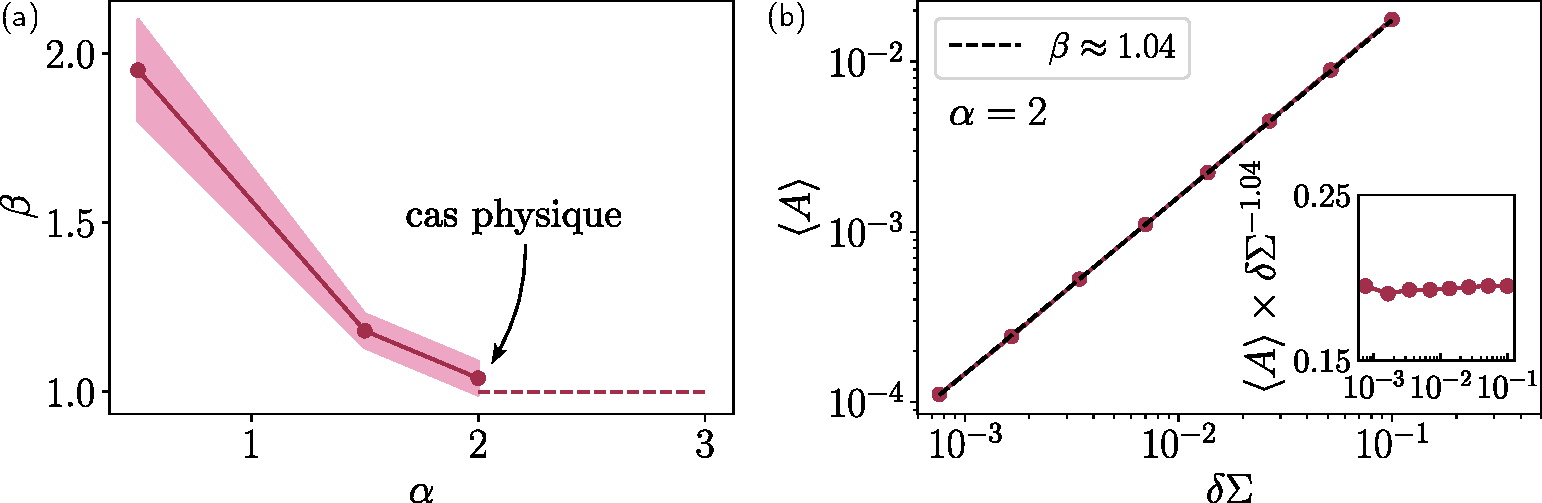
\includegraphics[width=\textwidth]{Chapitre5/Figures/DiscreteEPM.pdf}
	\caption{Résultats préliminaires obtenues dans le cadre du modèle élastoplastiques décrit à la \autoref{sec:EPMdiscret}. (a) Évolution de l'exposant $\beta$ avec la portée d'interaction $\alpha$. (b) Exemple de détermination de l'exposant $\beta$ dans le cas $\alpha = 2$ représentant le cas physique du propagateur d'Eshelby. Nous mesurons dans ce cas $\beta \approx 1.04$, ce qui est bien compatible avec les prédictions du modèle $\mu$-Hébraud-Lequeux avec $\mu = D/\alpha$ pour lequel on attend $\beta = 1$ avec des corrections logarithmiques \cite{lin_microscopic_2018}.}
	\label{fig:DiscreteEPM}
\end{figure}

\subparagraph{}In fine, dans le modèle $\alpha$-Picard, la zone d'influence du bruit interne semble être modifiée par les corrélations présentes dans le propagateur. Cette modification est illustrée par le texte \textit{corrélations} sur la \autoref{fig:Recap}-(c). Dans cette zone, le rôle des modes zéro semble être double : ceux-ci impliquent un signe alterné de la redistribution et donc la présence d'un bruit interne, et la forte anisotropie qu'ils induisent entraîne des corrélations d'activité qui rendent les propriétés de ce bruit hautement non-triviales.

\subsection{Limites du scénario proposé}

\subparagraph{}Si le scénario proposé pour interpréter l'évolutions de la criticalité des modèles $\alpha$-Picard et $\alpha$-ROM permet de mettre en évidence des différences intéressantes entre les deux phénomènes, celui-ci présente des limites et soulève quelques questions.

\subsubsection{Une approche découplée des mécanismes de création de l'activité}

\subparagraph{}Une hypothèse forte dans notre interprétation de ces transitions est de considérer les deux mécanismes de création d'activité (par transport ou par diffusion) de manière presque décorrélée. Nous discutons alors de quelques observations qui mettent en difficulté cette hypothèse dans le scénario que nous avons présenté.

\paragraph{$\alpha$-ROM}

\subparagraph{}Dans le $\alpha$-ROM, cette hypothèse est basée sur le fait que la borne $\alpha$ séparant le comportement de courte portée de la zone continue d'évolution des exposants se retrouve en $\alpha \approx D$ à deux et trois dimensions, exactement comme dans le cas du modèle $\mu$-Hébraud-Lequeux dans lequel la dynamique d'activité serait complètement triviale. Toutefois, si cette hypothèse de découplage entre les deux mécanismes semble validée par ce point, une incohérence se remarque dans les mesures de l'exposant de pseudo-gap $\theta$. En effet au \autoref{chapter:Susp} nous avons montré que l'exposant $\theta$, a priori contrôlé uniquement par le mécanisme de création de l'activité par diffusion, suit une évolution différente en fonction de la dynamique des particules actives (i.e. si celle-ci est décorrélée via des sauts infinis ou corrélée via des sauts finis). Cette observation suggèrerait donc que la dynamique des particules actives influence en fait la diffusion des particules passives. 

\subparagraph{}Aussi, dans le cas du $\alpha$-ROM en 2D nous mesurons $\theta \approx 0.75$ à $\alpha = 2$, qui marque le point de début de l'influence des interactions à longue portée sur le comportement critique. Or, si c'est le effectivement le mécanisme de création de l'activité par diffusion, seul,  qui permet de faire évoluer cette criticalité (comprendre sans influence du mécanisme de transport), nous nous attendrions à mesurer $\theta \approx 0.5$ à cette portée. En effet, il n'y a pas de raison de croire que le mécanisme de transport des particules actives puisse modifier, seul, l'exposant de pseudo-gap $\theta$ qui caractérise une structure à une échelle inférieure à la taille de sauts des particules actives.

\paragraph{$\alpha$-Picard}

\subparagraph{}Dans le cas du modèle $\alpha$-Picard, cette hypothèse est mieux motivée dans le scénario proposé. En effet, en présence d'un mécanisme de transport à longue portée, nous nous attendons dans une image naïve à ce que celui-ci prenne sa forme champ moyen ($\alpha = 3$ en 2D dans le cadre LR-CDP) bien avant que le mécanisme de diffusion via le bruit interne ne rentre en jeu ($\alpha = 2$ en 2D dans le modèle $\mu$-Hébraud-Lequeux avec $\mu = D / \alpha$). Toutefois, une observation assez inattendue est que, sur la base des mesures effectuée sur le modèle $\alpha$-Picard, l'exposant $\beta$ semble suivre une évolution assez monotone (voir \autoref{fig:Recap}-(b)), ne suggérant pas la présence d'un plateau $\beta = 1$ quelque part dans la zone entre $\alpha = 3$ et $\alpha = 2$. Ceci mériterait à être confirmé en mesurant $\beta$ finement dans cette zone, mais si cette observation persiste dans ce cas, le raccord parfait entre le régime LR-CDP et le régime $\mu$-Hébraud-Lequeux pourrait remettre en question le scénario que nous avons proposé.

\subparagraph{}Un autre point intéressant à remarquer est que dans la zone $\alpha < 3$ dans laquelle notre scénario, comme l'étude \cite{ferrero_criticality_2019}, suppose que le comportement peut être entièrement décrit par le modèle $\mu$-Hébraud-Lequeux (seulement avec $\mu \neq D/\alpha$), nous mesurons $2\theta \neq \beta$ qui est pourtant un attendu de cette image champ moyen. En effet, dans le cas des interactions d'Eshelby $\alpha = 2$ nous mesurons $\theta \approx 0.62$ et $\beta \approx 1.5$. Cette mesure est différente de celle présentée dans l'étude \cite{ferrero_criticality_2019} qui replace les modèles élastoplastiques avec $\alpha = 2$ dans le cadre $\mu$-Hébraud-Lequeux ($\theta \approx 0.75$) mais plus proche de celles présentées dans les études \cite{lin_scaling_2014, liu_driving_2016, lin_mean-field_2016} pour lesquelles on a clairement $\theta < 0.75$. Il pourrait alors être intéressant de mesurer cet exposant dans nos simulations d'une manière différente\footnote{Dans notre cas, nous avons évalué la distributions $P(x)$ dans les états élastiques issus des avalanches générées par le protocole RTP. Nous pourrions à la place procéder à une mesure sur des états actifs et mesurer $\theta$ via un redimensionnement par $\delta\Sigma$ comme on l'a fait dans le cas du $\alpha$-ROM} pour confirmer que l'on ait bien $\theta < 0.75$ et donc une déviation claire au cadre champ moyen du modèle $\mu$-Hébraud-Lequeux, ce qui fragiliserait le scénario présenté précédemment.

\subsubsection{Une vision réduite de la criticalité}

\subparagraph{}L'interprétation de l'évolution de la criticalité des modèles $\alpha$-Picard et $\alpha$-ROM que nous avons présentée présente un angle mort. En effet, celle-ci se base uniquement sur l'évolution de l'exposant $\beta$. Ceci se fait pour la raison principale que nous ne disposons pas en l'état des prédictions du modèle $\mu$-Hébraud-Lequeux concernant les autres exposants critiques comme $\gamma^\prime$, $\delta$\footnote{Dans certains cas, comme pour l'exposant d'hyperuniformité, ces prédictions sont impossibles du fait que la dynamique de type Hébraud-Lequeux est non spatialisée}. Dans le cas où ces prédictions sont réalisables, il serait donc intéressant de voir si la mesure numérique de ces autres exposants conforte le scénario proposé de la même manière que l'exposant de convexité $\beta$. Notamment il serait intéressant de parvenir à rationaliser l'évolution intriguante de l'exposant $\delta$ que nous avons mesuré dans le $\alpha$-ROM.

\subparagraph{}Pour remédier à ce problème, nous pourrions approfondir l'étude du modèle $\mu$-Hébraud-Lequeux, et éventuellement en proposer une version spatialisée afin de pouvoir définir dans ce cadre des exposants caractérisant des propriétés structurelles comme la dimension fractale des avalanches $d_f$ où l'exposant d'hyperuniformité $\alpha_\text{HU}$

\subsection{Vers un cadre théorique complet}

\subparagraph{}Afin de mieux comprendre l'évolution des criticalités présentées par les modèles $\alpha$-Picard et $\alpha$-ROM, un cadre d'interprétation théorique plus complexe serait donc nécessaire. Celui-ci permettrait notamment d'étudier conjointement l'effet des deux mécanismes de création de l'activité, par transport et par diffusion via le bruit interne. 

\subparagraph{}Dans le cadre LR-CDP, la compréhension de la criticalité et de son évolution avec $\alpha$ passe par la formulation d'équations de champ simples. Avec celles-ci et les méthodes de calculs adaptées, il est possible de déterminer le comportement critique à toutes les portées et en toute dimension. Il est donc tentant de vouloir établir une telle théorie dans le cadre des transitions observées dans les modèles $\alpha$-Picard et $\alpha$-ROM, capable de représenter les deux mécanismes de création de l'activité dans un même système d'équations en dimension finie. \`A la \autoref{sec:eqChampConv}, nous présentons le cheminement qui a occupé une période de cette thèse mais qui met en évidence les difficultés d'une telle formulation.

\section{Conclusion}

\subparagraph{}En conclusion, les transitions de réversibilité et d'écoulement étudiées à travers les modèles $\alpha$-Picard et $\alpha$-ROM présentent des similitudes frappantes. D'un point de vue constitutif, on y retrouve les mêmes ingrédients, similaires aux modèles de la classe CDP, et la présence d'interactions à longue portée ayant un effet spécifique. Celles-ci représentent un nouveau mécanisme de création de l'activité, associé à une diffusion vers une barrière. D'un point de vue phénoménologique global, les deux transitions présentent les mêmes évolutions montrant un comportement critique atypique à très longue portée et un comportement similaire à l'universalité CDP à très courte portée. Nous remarquons par ailleurs dans ces deux modèles la présence d'un point singulier mettant en lien le changement de convexité ($\beta = 1$), l'inversion du comportement des fluctuations critiques ($\gamma^\prime = 0$) et la perte de compacité spatiale des évènements dynamiques ($\chi = d_f = D$).


\subparagraph{}Toutefois, ces modèles présentent des points de divergence. Pour tenter de les expliquer, nous avons proposé un scénario basé deux cadres théoriques : le cadre LR-CDP qui rationalise l'influence du transport à longue portée et le cadre $\mu$-Hébraud-Lequeux qui rationalise l'effet du bruit interne sur le comportement critique. De manière générale, nous pouvons mettre en avant deux différences fondamentales. La première est que le $\alpha$-ROM ne présente jamais de transport de la quantité conservée à longue portée alors que c'est le cas du modèle $\alpha$-Picard. La seconde est que les modèles d'écoulement font intervenir une forme très particulière du propagateur, induisant des fortes corrélations dans le système tandis que le $\alpha$-ROM présente une dynamique simplifiée par le point de vue statistique adopté.

\subparagraph{}Enfin, nous avons évoqué les limites du scénario présenté pour rationaliser les évolutions et les différences constatées entre les modèles $\alpha$-Picard et $\alpha$-ROM. Pour passer outre celles-ci, une modélisation plus complète prenant simultanément en compte les mécanismes de création de l'activité par transport et par diffusion semble nécessaire. Cependant celle-ci semble être compliquée à déterminer.

%\subparagraph{}On pourrait s'interroger sur la possibilité que cette seconde différence vienne d'un défaut de modélisation et qu'une approche plus réaliste des interactions hydrodynamiques dans le $\alpha$-ROM permettrait de l'effacer. Toutefois, toute l'importance de la forme du propagateur dans le cas du modèle $\alpha$-Picard réside dans le fait que tous les évènements plastiques sont alignés avec la direction de cisaillement principale (i.e. le propagateur de Eshelby a une direction unique). Dans le cas de la transition de réversibilité, il n'y a pas de fortes raisons de penser que cette orientation soit privilégiée, et que si chaque interaction est orientée aléatoirement les corrélation spatiales du propagateur ne sont pas importantes. Dans la \autoref{sec:ApproxScalaire}, nous présentons des résultats préliminaires qui confortent la faible importance de ces corrélations dans le cas du modèle de particules en proposant un traitement tensoriel des interactions dans celui-ci.